
\chapter{Einführung}
\label{sec:intro}
	
	Im Laufe der Zeit werden immer mehr Prozesse digitalisiert bzw. 
	automatisiert - sei es in der Industrie, im zwischenmenschlichen 
	Bereich oder auch im Privathaushalt. Immer mehr Aufgabengebiete sollen vom 
	Menschen auf die Maschine übergehen, so auch der Vorgang des Sehens oder 
	auch des Erkennens von bestimmten Mustern. Dies ist für Industriebetriebe 
	insofern interessant, da es beispielsweise eine automatisierte 
	Identifizierung von Bauteilen anhand eines darauf eingravierten 
	Zeichencodes ermöglicht. Abbildung \ref{fig:example-code} zeigt 
	exemplarisch einen derartigen Code:
	\begin{figure}[h]
		\centering
		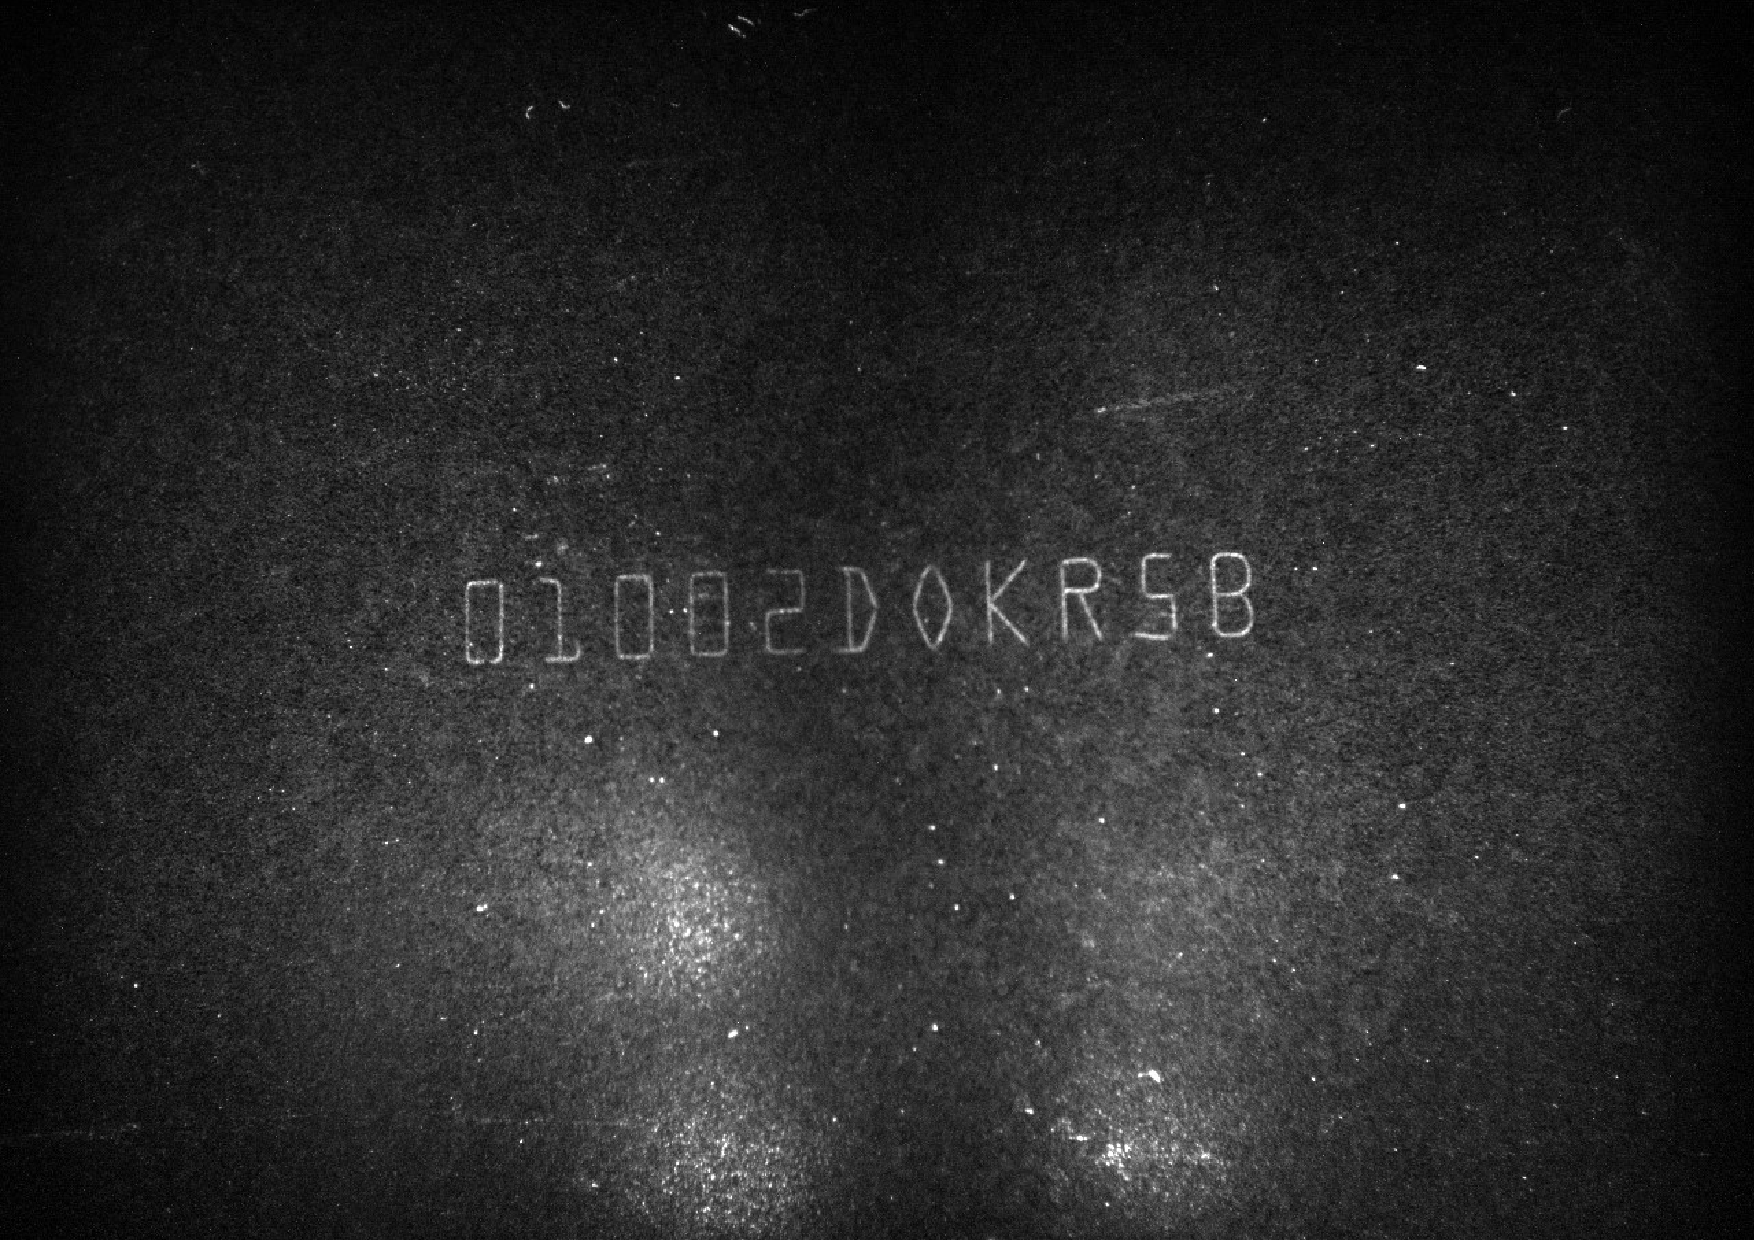
\includegraphics[width=0.5\linewidth]{beispielcode}
		\caption{Eingravierter Code auf metallischem Bauteil}
		\label{fig:example-code}
	\end{figure}
	
	
	
	Dabei ist innerhalb dieser Arbeit die folgende Struktur vorgesehen: \\
	Kapitel \ref{sec:prob} behandelt die 
